\subsection{Theseus: Environment--Data--Model Co-Evolution for RSI Intelligence}
\label{sec:practice_theseus}

% Inline brand logos for model--harness tables (assets under figures/logos/)
\newcommand{\theseuslogo}[1]{\raisebox{-2.2pt}{\includegraphics[height=7.5pt]{#1}}\hspace{0.25em}}
\newcommand{\openailogo}{\theseuslogo{figures/logos/openai_icon.png}}
\newcommand{\claudelogo}{\theseuslogo{figures/logos/claude_icon.png}}
\newcommand{\deepseeklogo}{\theseuslogo{figures/logos/deepseek_icon.png}}
\newcommand{\pilogo}{\theseuslogo{figures/logos/pi_icon.png}}
\newcommand{\glmlogo}{\theseuslogo{figures/logos/glm_icon.png}}
\newcommand{\kimilogo}{\theseuslogo{figures/logos/kimi_icon.png}}
\newcommand{\groklogo}{\theseuslogo{figures/logos/grok_icon.png}}
\newcommand{\metalogo}{\theseuslogo{figures/logos/meta_icon.png}}

\begin{table*}[!t]
    \centering
    \footnotesize
    \renewcommand{\arraystretch}{1.22}
    \caption{{Early workspace experiments in Theseus's environment stage. \textbf{(a)} Clean-versus-noise pilot: pass rates (\%) of eight frontier model--harness configurations on 30 workspace tasks with 1,280 rubrics, comparing a clean workspace against a noise-laden workspace. \textbf{(b)} Productivity study: rubric scores of five fixed harness--model pairings on 30 tasks with 547 rubrics, comparing the bare workspace against the reconstructed environment (a shared package of a Collection Map and an Event Log); ``Env.\ tasks'' reports wins/draws/losses at the task level, and ``Rubric flips'' counts rubrics that changed from fail to pass versus pass to fail.}}
    \label{tab:theseus_results}
    \vspace{0.3em}

    \textbf{(a) Clean-versus-noise pilot} --- clean vs.\ noise-laden workspace\\[0.35em]
    {\setlength{\tabcolsep}{6pt}
    \begin{tabularx}{\textwidth}{@{}>{\raggedright\arraybackslash}X l c c c@{}}
        \toprule
        \textbf{Model} & \textbf{Harness} & \textbf{Clean} & \textbf{Noise} & $\mathbf{\Delta}$ \textbf{(pp)} \\
        \midrule
        \deepseeklogo DeepSeek-V4-Pro   & \deepseeklogo DSH        & 98.2 & 46.6 & $+51.6$ \\
        \deepseeklogo DeepSeek-V4-Flash & \deepseeklogo DSH        & 90.1 & 63.7 & $+26.4$ \\
        \openailogo GPT-5.6-Sol         & \openailogo Codex        & 89.1 & 54.1 & $+35.1$ \\
        \glmlogo GLM-5.3                & \claudelogo ClaudeCode   & 88.8 & 57.2 & $+31.6$ \\
        \kimilogo Kimi-K3               & \claudelogo ClaudeCode   & 87.6 & 53.7 & $+33.9$ \\
        \groklogo Grok-4.6              & \claudelogo ClaudeCode   & 84.7 & 63.0 & $+21.7$ \\
        \openailogo GPT-5.6-Luna        & \openailogo Codex        & 84.6 & 38.1 & $+46.5$ \\
        \metalogo Muse-Spark-1.2        & \claudelogo ClaudeCode   & 84.5 & 53.3 & $+31.2$ \\
        \bottomrule
    \end{tabularx}}

    \vspace{0.6em}
    \textbf{(b) Productivity-workspace study} --- bare vs.\ reconstructed environment\\[0.35em]
    {\setlength{\tabcolsep}{3.2pt}
    \begin{tabularx}{\textwidth}{@{}>{\raggedright\arraybackslash}X l c c c c c@{}}
        \toprule
        \textbf{Harness} & \textbf{Model} & \textbf{Bare} & \textbf{Reconstructed} & $\mathbf{\Delta}$ \textbf{(pp)} & \textbf{Env.\ tasks} & \textbf{Rubric flips} \\
        \midrule
        \openailogo Codex CLI  & \openailogo GPT-5.6-Sol        & 60.51\% & 92.50\% & $+31.99$ & 24/3/3 & 190/15 \\
        \openailogo Codex CLI  & \deepseeklogo DeepSeek-V4-Flash & 54.30\% & 84.83\% & $+30.53$ & 24/3/3 & 201/34 \\
        \claudelogo Claude Code & \deepseeklogo DeepSeek-V4-Flash & 61.06\% & 79.71\% & $+18.65$ & 23/2/5 & 140/38 \\
        \pilogo PI             & \deepseeklogo DeepSeek-V4-Flash & 62.52\% & 89.03\% & $+26.51$ & 22/6/2 & 155/10 \\
        \pilogo PI             & \openailogo GPT-5.6-Sol        & 50.27\% & 89.95\% & $+39.67$ & 23/2/5 & 240/23 \\
        \bottomrule
    \end{tabularx}}

\end{table*}

\begin{figure*}[!t]
    \centering
    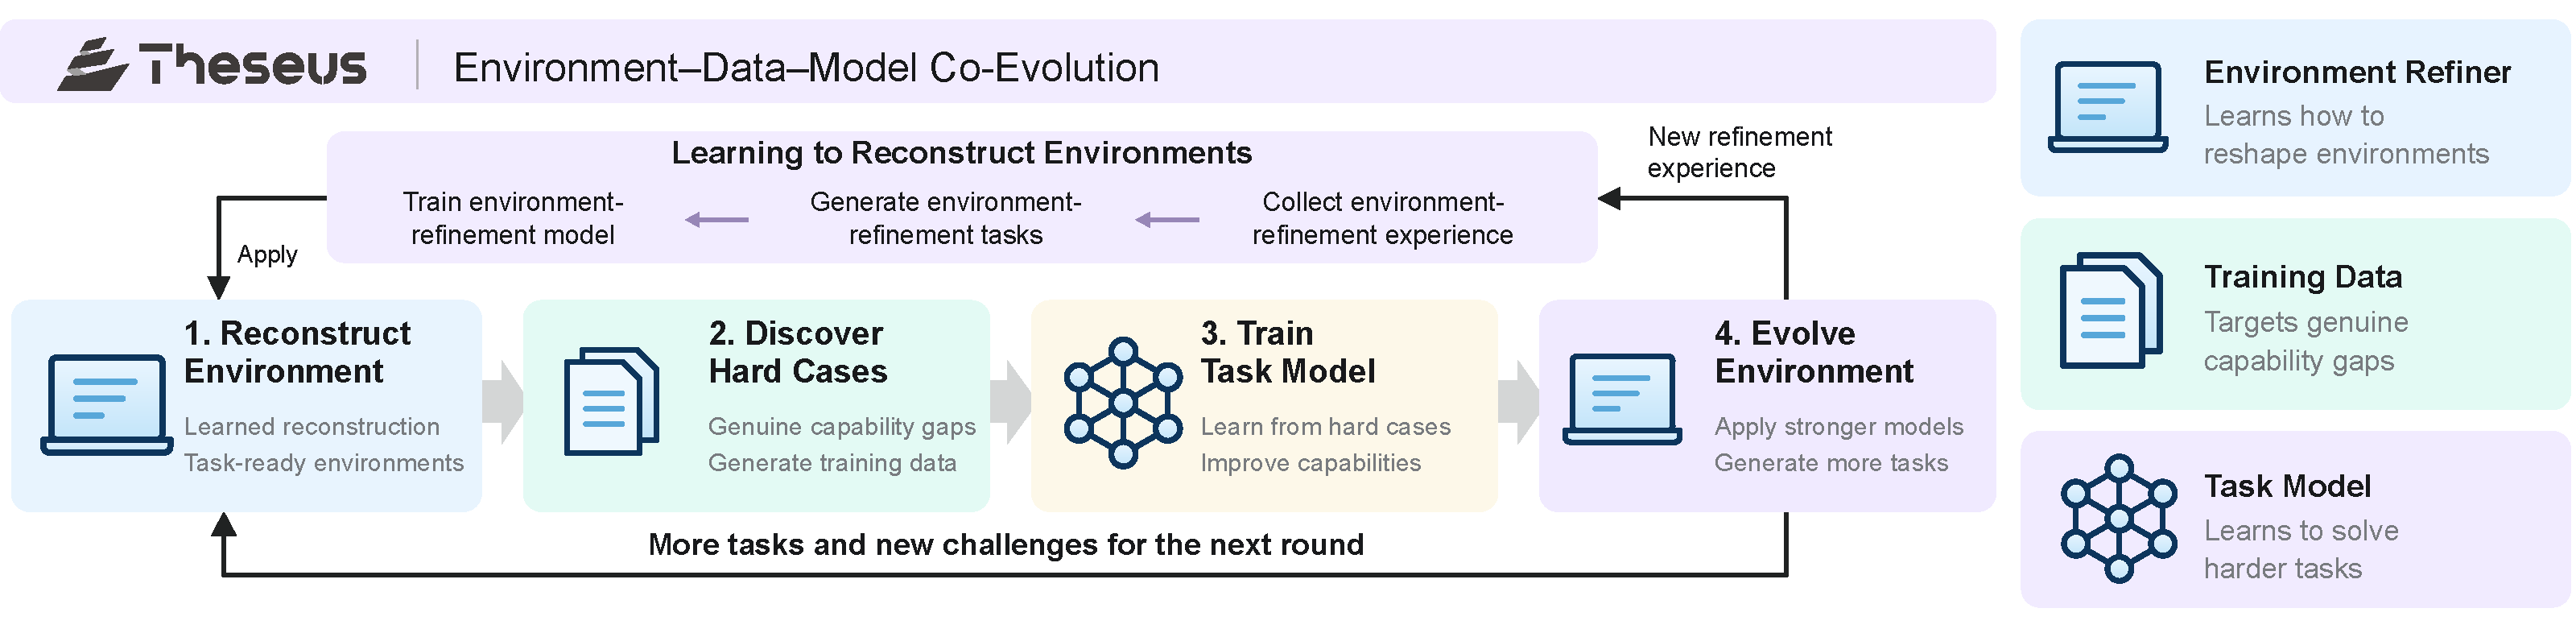
\includegraphics[width=\textwidth]{figures/Theseus.pdf}
    \caption{{Theseus's proposed four-stage co-evolution loop: reconstruct environments, uncover genuine capability gaps and generate training data, train task models, and iterate environments to produce more tasks. The upper loop learns an environment-refinement model from refinement experience and generated tasks, while successive iterations supply new experience for further refinement.}}
    \label{fig:bt_theseus}
\end{figure*}

{Theseus positions environment--data--model co-evolution as a path toward next-generation RSI intelligence. Its central premise is that environments make knowledge accessible and actions verifiable, task execution produces evidence for learning, and improved models expand the range of problems that can be explored. Under this vision, each round of work should contribute reusable capabilities to subsequent rounds, making real-world practice a continuing source of intelligence growth.} % \footnote{This case summarizes company-provided research and project materials current as of September 2026, including the working manuscript \emph{Hitting the Environment Wall: Evolving LLM Agent Workspaces for Recursive Self-Improvement}.}
%  progress should accumulate in the conditions that make future learning possible

{As shown in Figure~\ref{fig:bt_theseus}, Theseus realizes this vision in four steps. First, refinement experience is converted into environment-refinement tasks to train an environment-refinement model. Second, agents use reconstructed environments to identify genuine task-solving difficulties and generate targeted training data. Third, these data train the task model to improve its capabilities. Fourth, the stronger model supports further environment iteration and the generation of more tasks. Subsequent rounds yield both new task-training data and new environment-refinement experience, linking progress in solving tasks to progress in constructing the conditions for future learning.} % environment reconstruction becomes a learned capability: refinement experience is converted into 

{Early results provide an initial empirical basis for this direction in the workspace stage of the loop. A pilot with eight frontier model--harness configurations on 30 workspace tasks adapted from Workspace-Bench~\cite{tang2026workspacebench}, scored by 1,280 rubrics, first measured sensitivity to workspace quality: relative to a noise-laden workspace, a clean workspace raised pass rates by 21.7--51.6 percentage points across all eight configurations (Table~\ref{tab:theseus_results}a), suggesting that workspace state, rather than model capability alone, can bound agent performance. Building on this observation, a follow-up productivity study asked whether enriching the environment improves task performance while keeping the underlying model and harness fixed: five fixed model--harness pairings solved 30 tasks scored by 547 rubrics in total under a bare workspace and a reconstructed environment consisting of a Collection Map and an Event Log; the reconstructed environment raised aggregate rubric scores by 18.65--39.67 percentage points across all tested configurations (Table~\ref{tab:theseus_results}b), although a few tasks showed scope-creep regressions, where agents produced more extensive changes than the task required. The team has also completed training a reusable file-verification module. These early results mark the first steps of the co-evolution loop, and successive rounds will extend environment reconstruction, data generation, and model training into a sustained cycle of compounding improvement.}

%\wyk{Theseus's broader ambition is to make AI for Science a source of progress for future foundation models. Its project vision spans scientific frontiers including quantum computing, chemistry, controlled fusion, and brain science, where exploration can generate demanding tasks, testable hypotheses, and informative feedback. The intended relationship is reciprocal: stronger models advance scientific work, while scientific experience supplies knowledge and learning opportunities for subsequent models. Framed as an \emph{Evolution Model}, this agenda places sustained learning from practice at the center of model development and illustrates an environment-centered route toward RSI.}
